\begin{figure}
  \centering
  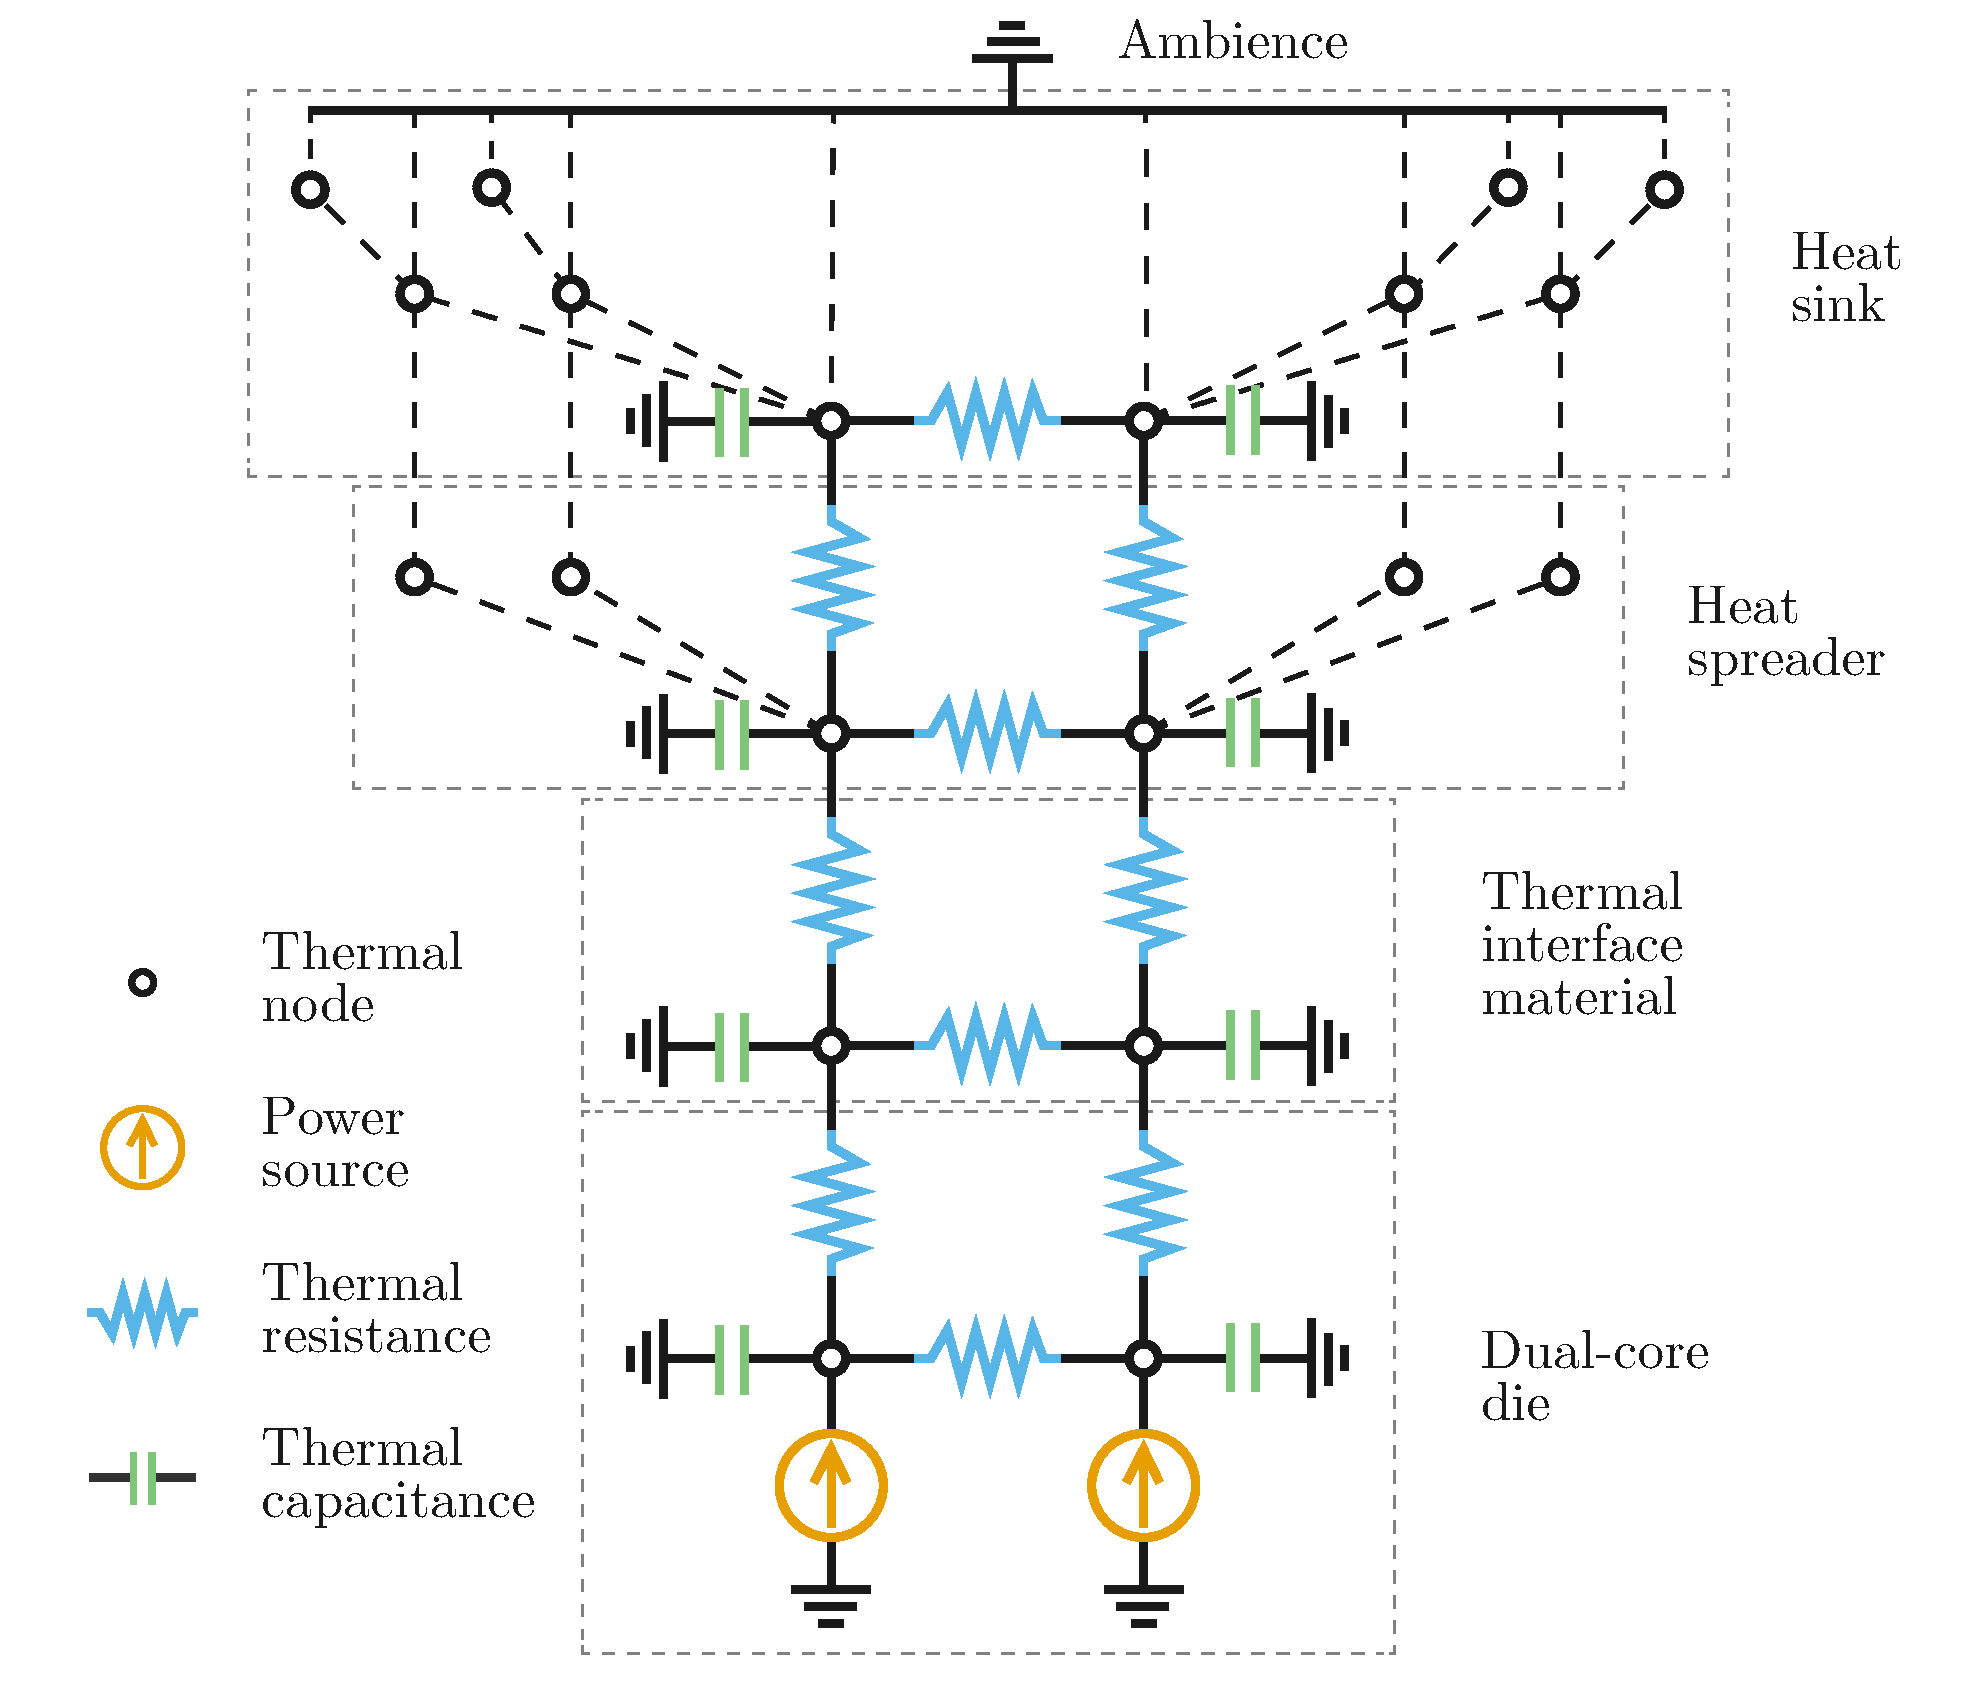
\includegraphics[width=\linewidth]{include/assets/circuit.pdf}
  \vspace{-1.0em}
  \caption{A simplified thermal RC circuit of a dual-core platform with a three-layer thermal package.}
  \flabel{circuit}
  \vspace{-1.5em}
\end{figure}

So far we have not made any assumptions regarding the cause of variability of the source term, \ie, the power term, in the thermal system given by \eref{fourier-system}.
In this section, we consider a particular application of the proposed framework.

\begin{figure*}
  \vspace{-1.0em}
  \centering
  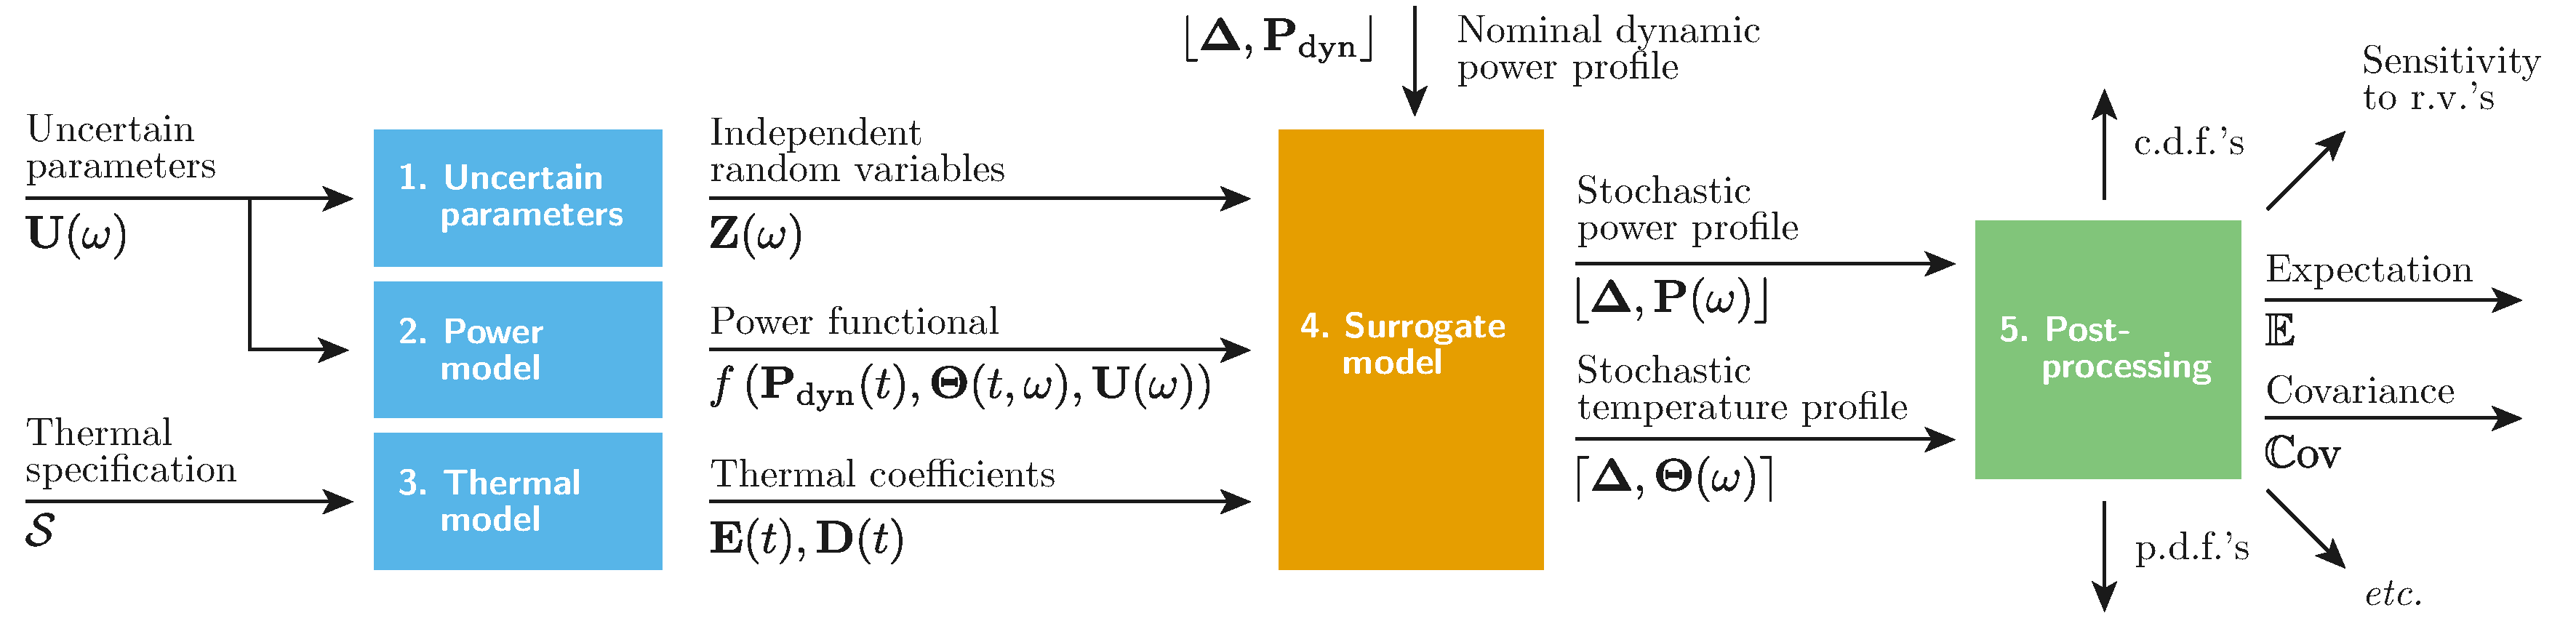
\includegraphics[width=1\textwidth]{include/assets/algorithm.pdf}
  \vspace{-1.0em}
  \caption{The structure of the proposed framework.}
  \flabel{algorithm}
  \vspace{-1.0em}
\end{figure*}

The probability space that we shall reside in is defined as a triple $(\outcomes, \sAlgebra, \pMeasure)$ where $\outcomes$ is a set of outcomes, $\sAlgebra \subseteq 2^\outcomes$ is a $\sigma$-algebra on $\outcomes$, and $\pMeasure: \sAlgebra \to [0, 1]$ is a probability measure \cite{maitre2010}.
Loosely speaking, an $n$-dimensional random variable is then a mapping $\v{X}: \o \in \outcomes \mapsto \v{X}(\o) \in \real^n$.
In what follows, the probability space $(\outcomes, \sAlgebra, \pMeasure)$ is always implied.

Consider a heterogeneous multiprocessor system that consists of $\nprocs$ processing elements and is equipped with a thermal package.
The processing elements are the active components of the system, \ie, those that dissipate power, identified at the intended level of granularity (processors, ALUs, caches, registers, \etc).
Let $\system$ be a thermal specification of the system defined as a collection of temperature-related information: (a) the floorplans of the active layers of the chip; (b) the geometry of the thermal package; and (c) the thermal parameters of the materials that the chip and package are made of.

A (transient) power profile $\profileP$ is defined as a tuple composed of a data matrix $\mP = (\vP_i) \in \real^{\nprocs \times \nsteps}$, $\vP_i \in \real^\nprocs$, that captures the power dissipation of the $\nprocs$ processing elements at $\nsteps$ moments of time and a (column) vector $\partition{\mP} = (\t_i) \in \real^{\nsteps}$ with positive and strictly increasing components that specifies these moments of time.
The definition of a (transient) temperature profile $\profileT$ is the same as the one for power except that the data matrix $\mTO$ contains temperature.

The system is assumed to depend on a set of uncertain parameters, denoted by a random vector $\vU(\o)$, $\o \in \outcomes$, which manifest themselves in deviations of the actual power dissipation from nominal values and, consequently, in deviations of temperature from the one corresponding to the nominal power consumption.
In what follows, we shall make a distinction between deterministic and stochastic profiles.
In the latter case, the power and temperature profiles are denoted by $\profileP{\o}$ and $\profileT{\o}$, respectively.

The goal of this work is to develop a probabilistic framework for power-temperature analysis (PTA) of multiprocessor systems where the actual power dissipation and temperature are stochastic due to their dependency on the set of uncertain parameters $\vU(\o)$.
The user is required to: (a) provide a thermal specification of the platform $\system$; (b) have prior knowledge (or belief) on the probability distribution of the uncertain parameters (\sref{uncertain-parameters}); and (c) specify a power model, in which $\vU(\o)$ is an input (\sref{power-model}).
The framework should provide the user with the tools to analyze the system under an arbitrary given workload and obtain the corresponding stochastic power $\profileP{\o}$ and temperature $\profileT{\o}$ profiles with a desired level of accuracy and at low costs.


\subsection{Uncertain Parameters} \slabel{ie-uncertain-parameters}
Independence of the parameters is a prerequisite of PC expansions.
In general, however, $\vU(\o)$ can be correlated and, therefore, should be preprocessed in order to fulfill the requirement.
To this end, an adequate probability transformation should be undertaken \cite{eldred2008}.
Denote such a transformation by $\vU(\o) = \oTransform{\vZ(\o)}$, which relates the correlated uncertain parameters $\vU(\o)$ with $\nvars$ independent random variables $\vZ(\o)$.

Correlated random variables can be transformed into uncorrelated ones \via\ a linear mapping based on a factorization procedure of the covariance matrix or covariance function of $\vU(\o)$; the procedure is known as the Karhunen-Lo\`{e}ve (KL) decomposition \cite{ghanem1991}.
If, in addition, the correlated variables form a Gaussian vector then the uncorrelated ones are also mutually independent.
In the general case (non-Gaussian), the most prominent solutions to attain independence are the Rosenblatt \cite{rosenblatt1952} and Nataf transformations \cite{li2008}.\footnote{Only a few alternatives are listed here, and such techniques as independent component analysis (ICA) are left outside of the scope of the paper.}
Rosenblatt's approach is suitable when the joint probability distribution function of the uncertain parameters $\vU(\o)$ is known; however, such information is rarely available.
The marginal probability distributions and correlation matrix of $\vU(\o)$ are more likely to be given, which are already sufficient for perform the Nataf transformation.\footnote{The transformation is an approximation, which operates under the assumption that the copula of the distribution is elliptical.}
The Nataf transformation produces correlated Gaussian variables, which are then turned into independent ones by virtue of the KL decomposition mentioned earlier.

Apart from the extraction of the independent parameters $\vZ(\o)$, an essential operation at this stage is model order reduction since the number of stochastic dimensions of the problem directly impacts the complexity of the rest of the computations.
The intuition is that, due to the correlations possessed by the random variables in $\vU(\o)$, some of them can be harmlessly replaced by combinations of the rest, leading to a smaller number of the variables in $\vZ(\o)$.
This operation is often treaded as a part of the KL decomposition.

In \sref{ie-uncertain-parameters}, we shall demonstrate the Nataf transformation together with the KL decomposition.
A description of the latter can also be found in the supplementary materials, \aref{karhunen-loeve}.


\subsection{Power Model} \slabel{ie-power-model}
In this section, we introduce the power model used in conjunction with the thermal model presented in \sref{thermal-model}. The total power dissipation of the system with $\cores$ processing elements is defined in the following abstract form:
\begin{equation} \elabel{power-model}
  \vP(\t, \o) = \f\Big(\vP_\dyn(\t), \vTO(\t, \o), \vZ(\o)\Big)
\end{equation}
where $\f: \real^\cores \times \real^\cores \times \real^\vars \to \real^\cores$ is an arbitrary function, possibly a ``black box'', of the nominal dynamic power $\vP_\dyn(\t)$, stochastic temperature $\vTO(\t, \o)$, and uncertain parameters $\vZ(\o)$. In this work, the function is assumed to be smooth in $\vZ(\o)$ and to have a finite variance, which is applicable to most physical systems \cite{xiu2002}. It can be seen that the definition of $\f$ provides a great flexibility to account for such effects as the well-known, strictly nonlinear interdependency between the leakage current and temperature \cite{srivastava2010, liu2007}. In this case, one can split the function into dynamic $\f_\dyn(\vP_\dyn(\t), \o)$ and leakage $\f_\leak(\vTO(\t, \o), \o)$ parts and define appropriate models for the components; this partition is to be further discussed in \sref{illustrative-example}.


\subsection{Thermal Models} \slabel{ie-thermal-model}
We move on to \stage{3}\ where the thermal model of the multiprocessor system is to be established.
Given the thermal specification $\system$ of the considered platform (the floorplan of the die, the configuration of the thermal package, \etc), we employ HotSpot (v5.02) \cite{hotspot} in order to construct the equivalent thermal RC circuits of the system.
Specifically, we are interested in the coefficient matrices $\mCF(\t)$ and $\mCS(\t)$ in \eref{fourier-system} (see also \fref{algorithm}), which HotSpot helps us to compute by providing the corresponding capacitance and conductance matrices of the system as described in \aref{thermal-model}.
In this case, thermal packages are modeled with three layers, and the relation between the number of processing elements and the number of thermal nodes is given by $\nnodes = 4 \nprocs + 12$.
An example of such a circuit for a dual-core platform is depicted in \fref{circuit}.

To conclude, the power and thermal models of the platform are now acquired, and we are ready to construct the corresponding surrogate model \via\ PC expansions.


\subsection{Surrogate Model} \slabel{ie-polynomial-chaos}
The goal is to transform the ``problematic'' term in \eref{recurrence}, \ie, the power term defined by \eref{power-model}, in such a way that the recurrence in \eref{recurrence} becomes computationally tractable. Our solution is the construction of a surrogate model for the power model in \eref{power-model}, which we further propagate through \eref{recurrence} to obtain an approximation for temperature. We employ the generalized polynomial chaos (PC) \cite{xiu2010}, which decomposes stochastic quantities into infinite series of orthogonal polynomials of \rvs. Such a series is especially attractive from the post-processing perspective as it is nothing more than a polynomial, hence, easy to interpret and evaluate. An introduction to orthogonal polynomials is given in \aref{orthogonal-polynomials}.

The first step towards a PC expansion is the choice of a suitable polynomial basis $\{ \pcb_i(\vz) \}$, which is typically picked from the Askey scheme of orthogonal polynomials \cite{xiu2010}. The step is crucial as the rate of convergence of PC expansions closely depends on it. There are no strict rules that guarantee the optimal choice \cite{maitre2010, knio2006}; however, there are best practices which say that one should be guided by the probability distributions of the \rvs\ that drive the stochastic system (see \aref{polynomial-chaos}). \tref{askey} in the appendix displays several examples of such paired probability distributions and polynomial bases. For instance, when the \rvs\ $\vZ(\o)$ follow a beta distribution, the Jacobi basis is worth being tried first. On the other hand, the Hermite basis (\fref{hermite}) is preferable for Gaussian \rvs.

Having an appropriate basis chosen, we apply the PC procedure to power in \eref{recurrence} and truncate the resulting infinite series in order to make it feasible for practical implementations. Such an expansion is formally defined as
\begin{equation} \elabel{pc-expansion}
  \oPC{\vars}{\pcorder}{\vP_k(\o)} = \sum_{i = 1}^{\pcterms} \pcc{\vP}_{ki} \; \pcb_i(\vZ(\o))
\end{equation}
where $\{ \pcb_i(\vZ(\o)) \}_{i = 1}^{\pcterms}$ is the truncated basis with $\pcterms$ polynomial terms of $\vars$ variables, and $\pcc{\vP}_{ki} \in \real^\cores$ are the coefficients of the expansion. The latter are computed using spectral projections as it is explained in the appendix, \aref{spectral-projection}. $\pcorder$ denotes the order of the expansion, which determines the maximal degree of the $\vars$-variate polynomials involved in the expansion; hence, $\pcorder$ also defines accuracy.

It can be seen in \eref{recurrence} that, due to the linearity of the operations involved in the recurrence, $\vX_k(\o)$ retains the same polynomial structure as $\vP_k(\o)$. Therefore, using \eref{pc-expansion}, \eref{recurrence} is rewritten as follows, for $k = 1, \dotsc, \steps$:
\begin{equation} \elabel{expanded-recurrence}
  \oPC{\vars}{\pcorder}{\vX_k(\o)} = \mCF_k \: \oPC{\vars}{\pcorder}{\vX_{k-1}(\o)} + \mCS_k \: \oPC{\vars}{\pcorder}{\vP_k(\o)}.
\end{equation}
Thus, there are two PC expansions for two concurrent stochastic processes with the same basis but different coefficients. As shown in \aref{spectral-projection}, \eref{expanded-recurrence} can be reduced to
\begin{equation} \elabel{pc-recurrence}
  \pcc{\vX}_{ki} = \mCF_k \: \pcc{\vX}_{(k - 1)i} + \mCS_k \: \pcc{\vP}_{ki}
\end{equation}
where $k = 1, \dotsc, \steps$ and $i = 1, \dotsc, \pcterms$. Finally, \eref{fourier-output} and \eref{pc-recurrence} are combined together to compute the coefficients of the PC expansion of the temperature vector $\vTO_k(\o)$.

To summarize, let us recall the stochastic recurrence in \eref{recurrence} where, in the presence of correlations, an arbitrary functional $\vP_k(\omega)$ of the uncertain parameters $\vU(\o)$ and random temperature $\vTO_k(\o)$ (see \sref{power-model}) needs to be evaluated and combined with another random vector, $\vX_k(\omega)$. Now, the recurrence in \eref{recurrence} has been replaced with a purely deterministic recurrence in \eref{pc-recurrence} that involves only linear operations. Moreover, the performed spectral decompositions have substituted the heavy thermal system in \eref{fourier-system} with a light polynomial surrogate defined by a set of basis functions $\{ \pcb_i(\vz) \}$ and the corresponding sets of coefficients, namely, $\{ \pcc{\vP}_{ki} \}$ for power and $\{ \pcc{\vTO}_{ki} \}$ for temperature, where $k$ traverses all the $\steps$ intervals $\dt_k$ of the considered time span. Consequently, the output of the proposed framework constitutes two stochastic profiles, the power $\profP{\o}$ and temperature $\profT{\o}$ profiles, that are ready to be analyzed from the UQ perspective.


\subsection{Post-processing} \slabel{ie-post-processing}
Due to the properties of PC expansions the obtained polynomial traces allow for
various prospective analyses to be performed with no effort. For instance,
consider the PC expansion of temperature at the $k$th moment of time given by
\begin{equation} \elabel{pc-k}
  \oPC{\nvars}{\pcorder}{\vTO_k} = \sum_{i = 1}^{\pcterms} \pcc{\vTO}_{ki} \pcb_i(\vZ)
\end{equation}
where $\pcc{\vTO}_{ki}$ are computed using \eref{fourier-output} and
\eref{pc-recurrence}. The expected value and variance have the following simple
expressions solely based on the coefficients:
\begin{equation} \elabel{pc-moments}
  \oExp{\vTO_k} = \pcc{\vTO}_{k1} \hspace{1em} \text{and} \hspace{1em} \oVar{\vTO_k} = \sum_{i = 2}^{\pcterms} \pcn_i \: \pcc{\vTO}_{ki}^2
\end{equation}
where the squaring should be understood elementwise. Such quantities as \cdfs,
\pdfs, probabilities of certain events, \etc\ can be estimated by sampling
\eref{pc-k}; each sample is a trivial evaluation of a polynomial.

